\chapter[Introdução]{Introdução}
% \addcontentsline{toc}{chapter}{Introdução}

De acordo com o Sistema de Informações sobre Mortalidade (SIM), entre 1980 e 2013, 106.093 mulheres foram vítimas de homicídio, representando em 2013 uma taxa de aproximadamente 13 homicídios femininos
diários \cite{mapa_violencia_2015}. 
No primeiro semestre de 2016 foram contabilizados 555.634 atendimentos na central de denúncias 
de violência contra a mulher, de acordo com o levantamento feito pela Secretaria de Políticas para as Mulheres (SPM). 
Aproximadamente 54\% dos atendimentos foram para prestação de informações. De acordo com \cite{portal_180}, aproximadamente 13\% dos atendimentos, são relatos de violência física (51\%), psicológica (31,1\%), moral (6,51\%), patrimonial (1,93\%), sexual (4,30\%), cárcere privado (4,86\%) e tráfico de pessoas (0,24\%).

Cenários como esse impulsionaram o governo à criação de políticas públicas (PP) 
nacionais para a redução da violência contra as mulheres, como a criação de leis (Lei Maria da Penha, Lei do Feminicídio)
e de estratégias de apoio às mulheres e de conscientização da população. Além disso, estratégias tecnológicas, como aplicativos e sites, têm sido apoiadas pelo governo e criadas pela própria população. 


\section{Objetivo}
O objetivo do trabalho é propor uma \textit{Application Programming Interface} (API) para uso em sistemas de tomada de decisão e planejamento de segurança para mulheres vítima de violência. 
% Para realização da proposta os objetivos específicos
% do trabalho são:
% \begin{itemize}
% 	\item Compreender os sistemas existentes de apoio à mulheres vítima de violência;
% \end{itemize}


% Na Figura \ref{fig:sistemas_categorizados} são apresentados algumas aplicações criadas para apoio à mulher vítima
% de violência em cinco categorias: Levantamento de Dados e estatísticas, Mapeamento de riscos, Informativos, Pedido de Socorro e Apoio.


% \begin{figure}[ht]
% \centering
% 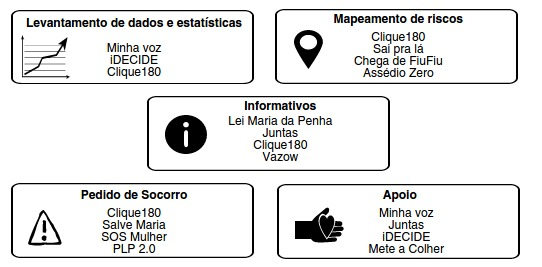
\includegraphics[scale=0.85]{figuras/sistemas_relacionados.jpeg}
% \caption{Aplicações de apoio à mulher vítima de violência}
% \label{fig:sistemas_categorizados}
% \end{figure}


